%Created on: May 21, 2014        Edited by: Wesley Kyle
%Edited on: May 20, 2016        Edited by: P. Gimby - replaced preamble with input from external file
%Edited on: Aug 23, 2016        Edited by: W.Kyle - Corrected typos and formating issues

% Beginning code for all standard physics latex documents

%Created on: May 8, 2014    Edited by: Wesley Kyle
%Edited on:	May 12, 2016	Edited by: P. Gimby - cleaned up the code to remove unneeded packages
%Edited on:	May 13, 2016	Edited by: P. Gimby - collected a few more packages used in 325.
%Edited on:	May 16, 2016	Edited by: P. Gimby - fixed page numbering error.
%Edited on: May 20, 2016	Edited by: Alex Shook - Added packages for 497

\documentclass[justified]{tufte-book}
\usepackage{graphicx} % allow embedded images
\setkeys{Gin}{width=\linewidth,totalheight=\textheight,keepaspectratio}
\usepackage{amsmath}  % extended mathematics
\usepackage{bm}  % bold font in math mode
\usepackage{longtable} %lets long tables flow into multiple pages instead of running off the page or having to break tables up manually
\usepackage{booktabs} % book-quality tables
\usepackage{units}    % non-stacked fractions and better unit spacing
\usepackage{multicol} % multiple column layout facilities
\usepackage{tikz} %for drawing nice pictures
\usepackage{indentfirst} % makes first line of each new section be indented
\usepackage{enumitem} % extended options for the enumerate environment
\usepackage{soul} % gives more typestting options like spacing, underline, and strike-through
\usepackage{marvosym} %extra symbols package
\usepackage{multirow} % for special table controls
\usepackage[singlelinecheck=false]{caption} % allow captions w/o figure number
\captionsetup{compatibility=false} % corrects in issue with the caption package
\usepackage{float} % allows for contorl over position of figures and tables
\allowdisplaybreaks % allows equations to span two pages if needed
\usepackage{mathrsfs} % fancy math symbols
\usepackage{multirow} % for special table controls
\usetikzlibrary{arrows,shapes,snakes,calc,patterns,3d} % addon to tikz
\usetikzlibrary{circuits.ee.IEC} % addon to tikz
\usepackage{pgfplots} % package for making plots of functions
\usepackage{gensymb} % symbols i,e. degrees
\usetikzlibrary{decorations.pathmorphing} % to draw the springs
\tikzset{circuit declare symbol = ac source}
\tikzset{set ac source graphic = ac source IEC graphic}
\usepackage{changepage} % allows for full page environment
\usepackage{comment} % allows comment tags for large sections

% define new page style that puts page numbers in the middle
%\begin{comment}
\fancypagestyle{custom}{
\fancyhf{} % clear all header and footer fields
\fancyheadoffset{0pt}
\fancyfootoffset{0pt}
\fancyfoot[C]{\thepage}
\renewcommand{\headrulewidth}{0pt}
\renewcommand{\footrulewidth}{0pt}}
\pagestyle{custom}
%\end{comment}

%below creates a new circuit symbol for AC sources
\tikzset{
         ac source IEC graphic/.style=
          {
           transform shape,
           circuit symbol lines,
           circuit symbol size = width 3 height 3,
           shape=generic circle IEC,
           /pgf/generic circle IEC/before background=
            {
             \pgftransformresetnontranslations
             \pgfpathmoveto{\pgfpoint{-0.8\tikzcircuitssizeunit}{0\tikzcircuitssizeunit}}
             \pgfpathsine{\pgfpoint{0.4\tikzcircuitssizeunit}{0.4\tikzcircuitssizeunit}}
             \pgfpathcosine{\pgfpoint{0.4\tikzcircuitssizeunit}{-0.4\tikzcircuitssizeunit}}
             \pgfpathsine{\pgfpoint{0.4\tikzcircuitssizeunit}{-0.4\tikzcircuitssizeunit}}
             \pgfpathcosine{\pgfpoint{0.4\tikzcircuitssizeunit}{0.4\tikzcircuitssizeunit}}
             \pgfusepathqstroke
            }
          }
        }
% end of circuit symbol
%\begin{document}
%%%end individual beginning code/,$d


%  \begin{titlepage}
%    \vspace*{\fill}
%    \begin{center}
%      \huge{{\bf TITLE1}}\\[0.4cm]
%      \huge{TITLE2}\\[0.4cm]
%      \LARGE{Laboratory Manual}\\[0.4cm]
%      \large{SEASON YEAR}
%    \end{center}
%    \vspace*{\fill}
%  \end{titlepage}
%\maketitle

%\begin{spacing}{0.5}
%\tableofcontents
%\end{spacing}

%NEW PHYS 497 PACKAGES AND COMMANDS

%Subcaption package: Allows subfigures to be placed side by side, and labeled with individual captions (Added June 1, 2016)
\usepackage{subcaption}

%Array package: Allows for addiation specifications in arrays (Added May 6, 2016)
\usepackage{array}

%newcolumntype: Allows one to specify a fixed column width (Added May 6, 2016)
\newcolumntype{L}[1]{>{\raggedright\let\newline\\\arraybackslash\hspace{0pt}}m{#1}}
\newcolumntype{C}[1]{>{\centering\let\newline\\\arraybackslash\hspace{0pt}}m{#1}}
\newcolumntype{R}[1]{>{\raggedleft\let\newline\\\arraybackslash\hspace{0pt}}m{#1}}

%circuits.logic.US, circuits.logic.IEC: For drawing logic gates in Tikz (Added May 6, 2016) 
\usetikzlibrary{circuits.logic.US,circuits.logic.IEC}

\newcommand{\PGT}{ %PGT: positive going transition
\begin{tikzpicture}
\draw[-angle 60] (0,0) -- (0,5pt);
\draw (0,5pt) -- (0,6pt) -- (5pt,6pt);
\draw (-5pt,0) -- (0,0);
\end{tikzpicture}
}





%TEST
\usepackage{geometry}
\pagestyle{fancy}

%\usepackage[caption=false]{subfig}

%\makeatletter
%\renewenvironment{figure}[1][htbp]{%
%  \@tufte@orig@float{figure}[#1]%
%}{%
%  \@tufte@orig@endfloat
%}

%\renewenvironment{table}[1][htbp]{%
%  \@tufte@orig@float{table}[#1]%
%}{%
%  \@tufte@orig@endfloat
%}
%\makeatother

% use instead of subfigure
\makeatletter
\newenvironment{multifigure}[1][htbp]{%
  \@tufte@orig@float{figure}[#1]%
}{%
  \@tufte@orig@endfloat
}
\makeatother

\makeatletter
\newenvironment{mainfigure}[1][htbp]{%
\@tufte@orig@float{figure}[#1]
\begin{adjustwidth}{}{-153pt}}
{\end{adjustwidth}\@tufte@orig@endfloat}%
\makeatother

\makeatletter
\newenvironment{maintable}[1][htbp]{%
\@tufte@orig@float{table}[#1]
\begin{adjustwidth}{}{-153pt}}
{\end{adjustwidth}\@tufte@orig@endfloat}%
\makeatother

%%%% Labatorial Cross-over labs need this code. This should be temporary PG Dec 7, 2016

\newcounter{questioncounter}
\setcounter{questioncounter}{0}
\newcounter{checkpointcounter}
\setcounter{checkpointcounter}{0}
\newcounter{figurecounter}
\setcounter{figurecounter}{0}
%%%%%%%%%%%%%%%%%%%%%%%%%%%%%%%%%%%%%%%%%%%%%%%%%%%%%%%

\newcommand{\checkpoint}{
 \fbox{\begin{minipage}{0.2\textwidth}
 %\includegraphics[width=0.5\textwidth]{stop}
 \end{minipage}
 \begin{minipage}{1.0\textwidth}
 {\bf CHECKPOINT \addtocounter{checkpointcounter}{1} \arabic{checkpointcounter}: Before moving on to the next part, have your TA check the results you obtained so far.}
 \end{minipage}}}

%%% end labatorial cross-over code.

% New environment for placing figure captions under the figure
%\makeatletter
%\newenvironment{mainfigure}{\textwidth}[1][htbp]{%
%\@tufte@orig@float{figure}[#1]%
%}{%
%\@tufte@orig@endfloat
%}
%\makeatother


\begin{document}

%%%start document%%% DO NOT REMOVE THIS LINE

\chapter{Vacuum Technology Laboratory}

The production of low-pressure environments is important for many research activities because it isolates an experiment from the surroundings. This is essential because some materials react if exposed to air, either by slow oxidation or something more violent. In other cases, it is a process, such as thin layer deposition, which is affected by the presence or lack of air. Often it is thermal isolation that is being sought and there is no more efficient thermal insulator than a perfect vacuum. In optical sciences, certain wavelength regions, referred to as the vacuum ultraviolet, extreme ultraviolet, and parts of the far infrared region, employ photons that are absorbed by air. It would not be possible to work in these regions without a good vacuum system. Other optical processes are disguised or even destroyed by rapid collisions with air molecules, and thus high vacuum is needed. In summary, many studies in atomic and molecular, condensed matter, laser, nuclear, optical, particle, plasma, and quantum physics are only possible with the use of vacuum systems. In addition, many applied areas such as thin film deposition, and etching are possible only at low pressures.

Working with vacuum systems is interesting and challenging. The equipment is often easily damaged, and in some cases, specifically when working with liquid nitrogen, can be somewhat hazardous to its operators. Please ask your TA for help if you are at all unsure of what you are doing. We will be happy to show you how to work the equipment, more than once if needed, and we don't want to see either you or the equipment hurt.

When working with glass equipment, take care that you never use too much force opening or closing valves, and keep metal and heavy objects away from the glass parts, we don't want any breakages. When working with pumps, don't expose them directly to atmospheric pressure while they are operating. Only rotary pumps and pumping lines should be filled with air immediately after turning the pump off. Both diffusion pumps and sorption pumps are thermal pumps and should not be exposed to air while they are operating. Even after you have turned off the heat or removed the cooling nitrogen, these pumps take some time to change temperature, so they should be left sealed off from the lab throughout this process. Finally, when handling liquid nitrogen, you must take care not to spill this very cold liquid onto material that will absorb the liquid and hold it in contact with your skin. A small amount spilled on bare skin should not cause a problem, but spilling it onto clothing such as sweaters can lead to burns. Therefore, you should roll up your sleeves if you are working with liquid nitrogen. In summary, we ask you to be careful.  When in doubt, ask your TA or instructor for assistance.

For each experiment, you will make some observations or measurements and record these in your lab notebook. The observations or data that must be recorded in the lab notebook are indicated in {\bf bold type} in the experimental procedures accompanying each experiment.

\section{I - Mechanical Gauges and Pumps}

\section{Equipment}

% first column
\begin{minipage}[t]{0.5\textwidth}
\begin{itemize}[noitemsep]
\item Schematic diagram of vacuum pump principles
\item Hand operated vacuum pump
\end{itemize}
\end{minipage}
%second column
\begin{minipage}[t]{0.5\textwidth}
\begin{itemize}[noitemsep]
\item Edwards RV5 mechanical pump
\item board-mounted gauges (5)
\end{itemize}
\end{minipage}

\begin{marginfigure}
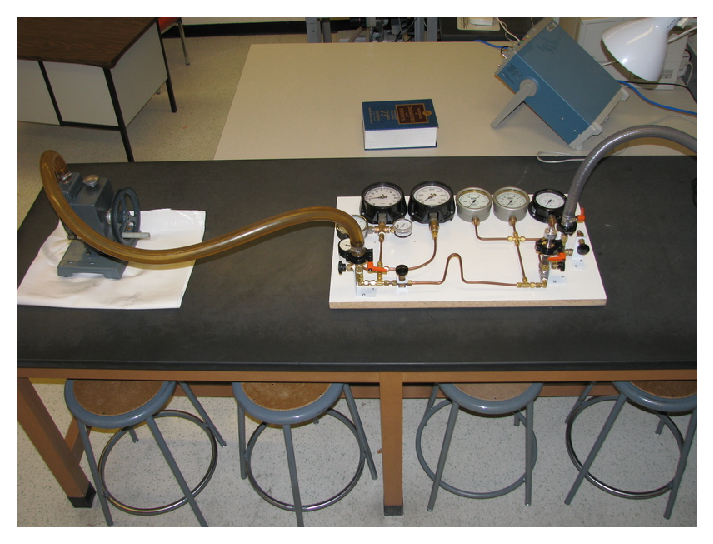
\includegraphics{Mechanical-Gauges-and-Pumps-Table8.eps}
\caption{Mechanical Gauges Setup}
\label{fig:VACsetup1}
\end{marginfigure}

\section{Introduction}

Mechanical gauges are relatively simple and inexpensive devices used to measure the pressure inside a chamber or gas line. They are equally adept at measuring pressures either above (high pressure) or below (vacuum) atmospheric pressure. Examples of mechanical gauges designed to measure high pressure can be found on the regulator of the helium tank that is used in the "Leaks and Leak Detection" experiment. The "Mechanical Gauges and Pumps" will introduce you to mechanical gauges used to measure pressures in vacuum systems.

Mechanical gauges operate by comparing the pressure inside the vessel to which they are attached, to the pressure outside the gauge, i.e. the pressure in the room in which you are working. Consider a piston with springs attached to each side, as shown in Fig. \ref{fig:vac1}. One side of the piston is open to the experimental chamber and the other to the lab room. When the chamber pressure is above room or atmospheric pressure, the gauge reads a positive value. When the room pressure is higher, the piston is pushed to the left, resulting in a negative number. This design has led to the terminology of gauge pressure and absolute pressure. Absolute pressure is the pressure relative to zero force or zero particles. It is the true pressure generated by a gaseous sample. Gauge pressure, on the other hand, is the pressure measured relative to 1 atmosphere. To convert from gauge pressure to absolute pressure, simply add 1 atmosphere to the gauge pressure value.

\begin{figure}
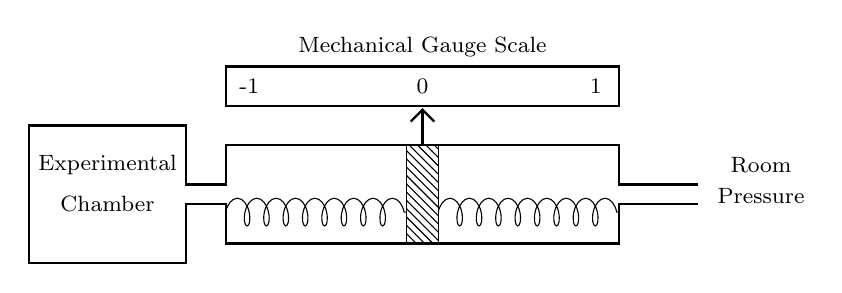
\begin{tikzpicture}
\draw[thick](9,4.75)--(8,4.75)--(8,5.25)--(3,5.25)--(3,4.75)--(2.5,4.75)--(2.5,5.5)--(.5,5.5)--(.5,3.75)
--(2.5,3.75)--(2.5,4.5)--(3,4.5)--(3,4)--(8,4)--(8,4.5)--(9,4.5);
\draw[decorate,decoration={coil,segment length=7pt,amplitude=5pt}](3,4.4)--(5.3,4.4);
\draw[decorate,decoration={coil,segment length=7pt,amplitude=5pt}](5.7,4.4)--(8,4.4);
\draw[pattern=north west lines](5.3,4)rectangle(5.7,5.25);
%mechanical gauge scale
\draw[thick](3,5.75)rectangle(8,6.25);
\draw[thick](5.35,5.55)--(5.5,5.7)--(5.65,5.55); % indicator arrow
\draw[thick](5.5,5.25)--(5.5,5.7); % indicator arrow
%labels
\node[font=\footnotesize]at(1.5,5){Experimental};
\node[font=\footnotesize]at(1.5,4.5){Chamber};
\node[font=\footnotesize]at(5.5,6.5){Mechanical Gauge Scale};
\node[font=\footnotesize]at(3.3,6){-1};
\node[font=\footnotesize]at(5.5,6){0};
\node[font=\footnotesize]at(7.7,6){1};
\node[font=\footnotesize]at(9.8,5){Room};
\node[font=\footnotesize]at(9.8,4.6){Pressure};

\end{tikzpicture}
\caption{Schematic representation of a mechanical gauge.}
\label{fig:vac1}
\end{figure}

This type of mechanical device has an interesting effect on pressure measurements. When using a regular mechanical gauge, the value that the gauge reads is dependent on the actual atmospheric pressure. In other words, if a storm front moves through the city that you are working in, the reading on your mechanical pressure gauge will change. 

There are a variety of pressure units in common usage throughout the scientific and industrial communities. Table 1 summarizes some of the commonly used units.

\begin{figure}
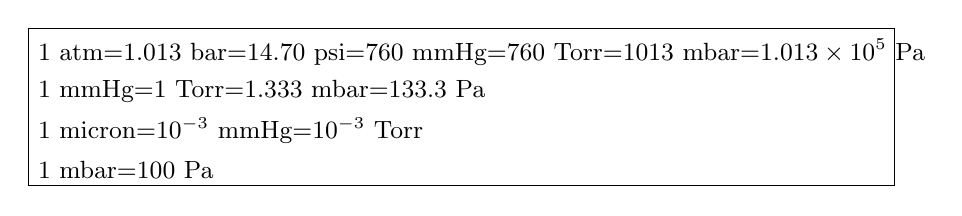
\begin{tikzpicture}
\draw(0,0)rectangle(11,2);
\node[right,font=\small]at(0,1.7){1 atm=1.013 bar=14.70 psi=760 mmHg=760 Torr=1013 mbar=$1.013\times10^5$ Pa};
\node[right,font=\small]at(0,1.2){1 mmHg=1 Torr=1.333 mbar=133.3 Pa};
\node[right,font=\small]at(0,.7){1 micron=$10^{-3}$ mmHg=$10^{-3}$ Torr};
\node[right,font=\small]at(0,.2){1 mbar=100 Pa};
\end{tikzpicture}
\normalsize

%\stepcounter{figure}
\smallskip\noindent Table 1: Some commonly used pressure units and conversions.
\end{figure}

There are two general types of mechanical gauge scales used with vacuum systems.  The first is the one discussed above, where the gauge is measuring gas pressure. In general, a zero reading (atmospheric) is in the middle of the scale. As a chamber is pumped out, the needle wraps counterclockwise indicating more and more negative gauge pressures. Some pressure gauges read "absolute" pressure by labeling the position of the needle when chamber and room pressures are equal at 14.7 psi or 760 Torr. The negative side of the gauge then counts down towards zero pressure. Can you see the problem that this can cause, especially for labs that are not at sea level? The alternate set-up that is often found is a vacuum gauge. This type of gauge measures the amount of "vacuum" that has been generated. At room pressure, the gauge reads zero. Then, as you pump out the chamber, the needle wraps clockwise, indicating that more and more vacuum is being generated. It is somewhat odd terminology, but is still used. This system is designed to allow you to look at both a vacuum gauge and a pressure gauge.

\section{Experimental Procedure}
\begin{enumerate}
\item The experimental apparatus for this system is quite simple. It consists of a small hand-operated rotary vacuum pump and a motor-driven pump. The pumps are connected to several mechanical gauges, including both vacuum and pressure gauges. Examine the pump unit to ensure that you are going to turn the handle in the correct direction as indicated by the arrow on the side of the pump. Turn the handle slowly and observe the mechanism through the Plexiglas plate. Do you understand how the pump works?

\item Open the valve to the gauge assembly and use pump air out of the system with the hand-operated pump. Watch the gauge readings as the system is evacuated. How fast does this occur? Are there any differences in the behaviours of the gauges? 

\item Once the pressure has reached a final steady-state value, close the valve to the pump. Examine the values of the gauges. Do the values on the different gauges make sense, both with respect to one another and with respect to the atmospheric pressure? You might want to consult Table 1 for conversions between different units.

\item What is the effect of the fact that Calgary is roughly 1000 m above sea level? Using the mercury barometer located in the lab, record the atmospheric pressure in the laboratory. Ask your TA for help to use this device. {\bf In your lab notebook, record the absolute pressure measured by one of the gauges in the assembly and the relative pressure recorded by on of the gauges in the assembly. Do the gauge pressures and the atmospheric pressure in the laboratory reconcile with each other?}

\item Let air back into the system. Then, try pumping the system at different speeds with the hand-operated pump. What is the effect of the speed on the ultimate pressure that you can achieve?

\item Close the vent valve and evacuate the gauge assembly using the motor-driven rotary vane mechanical pump. {\bf In your lab notebook, record the absolute pressure measured by one of the gauges in the assembly and the relative pressure recorded by on of the gauges in the assembly. How do these pressures compare with those recorded in Step 4?}

\item When you are finished measuring the pressures on the gauges, isolate the rotary vane mechanical pump from the gauge assembly and vent the entire system back to atmospheric pressure.
\end{enumerate}

\section{II - Pumping With No Moving Parts}

\section{Equipment}

% first column
\begin{minipage}[t]{0.5\textwidth}
\begin{itemize}[noitemsep]
\item Sorption pump
\item Liquid nitrogen dewar
\end{itemize}
\end{minipage}
%second column
\begin{minipage}[t]{0.5\textwidth}
\begin{itemize}[noitemsep]
\item thermocouple vacuum gauge
\end{itemize}
\end{minipage}

\begin{marginfigure}
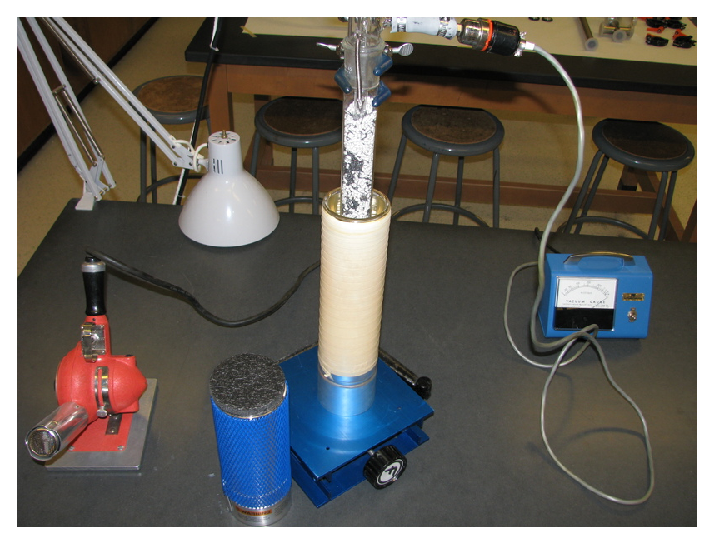
\includegraphics{Sorption-Pump-Table3.eps}
\caption{Sorption Pump Setup}
\label{fig:VACsetup2}
\end{marginfigure}

\section{Introduction}

The vast majority of all techniques that are used to evacuate gases from containers use some form of moving parts to accomplish this feat. In some cases, such as rotary mechanical, turbo molecular, and roots blower pumps, the moving parts are mechanical, generally rotating vanes that push and compress the gases, forcing them out of the vessel. In other cases, such as the Diffstak and glass diffusion pumps it is gets of gas that are directed to push all the atoms and molecules out of the chamber. However, there is one exception to all of these techniques.  These are the cryogenic pumping techniques, which use condensation and absorption of atoms and molecules to remove gas particles from an evacuated chamber. The example that you will meet here is a Sorption Pump. Sorption pumps use liquid nitrogen cooled 'molecular sieve' material to condense and absorb atoms or molecules. Molecular sieve is a chemical that is designed to have a large surface area and a large number of small openings throughout its structure, which are just the correct size to trap selected atoms or molecules.

\begin{marginfigure}
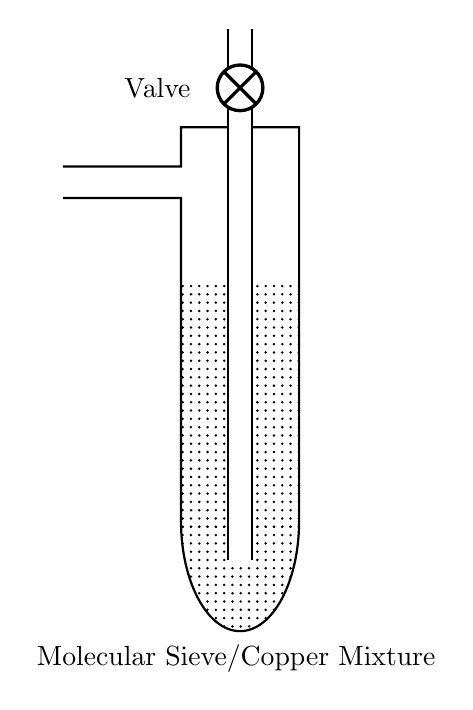
\begin{tikzpicture}
\draw[pattern=dots,draw=white](2,1.4)rectangle(3.5,4.5); %holes in sieve
\draw[draw=white,pattern=dots](3.5,1.5)arc(0:-180:.75 and 1.4)--(3.5,1.5); %holes in sieve
\draw[thick](.5,6)--(2,6)--(2,6.5)--(3.5,6.5)--(3.5,1.5)arc(0:-180:.75 and 1.4)
--(2,5.6)--(.5,5.6);
\draw[draw=white,fill=white](2.6,1)rectangle(2.9,7.75); %straw
\draw[thick](2.6,1)--(2.6,7.75); %straw
\draw[thick](2.9,1)--(2.9,7.75); %straw
\node[circle,draw,very thick,scale=1.75,fill=white]at(2.75,7){};
\draw[very thick](2.55,6.8)--(2.95,7.2);
\draw[very thick](2.95,6.8)--(2.55,7.2);
%labels
\node[]at(1.7,7){Valve};
\node[]at(2.7,-.25){Molecular Sieve/Copper Mixture};
\end{tikzpicture}
\caption{Sketch of a sorption pump assembly.}
\label{fig:vac2}
\end{marginfigure}

The Sorption pump shown in Fig. \ref{fig:vac2} consists simply of a long glass tube with two connectors positioned near the top of the tube. The tube is completely enclosed other then these two opening, to which are generally connected vacuum tubes. The tube is filled with a mixture of molecular sieve and copper strands. The molecular sieve material does the pumping, while the copper is there principally to ensure that the entire system is at a uniform temperature. The top vacuum connection is actually a long tube that goes down the middle of the tube through the pumping material to its opening near the bottom of the tube. The top of the glass tube is removable to allow for addition or replacement of the molecular sieve/copper filament mixture.

\section{Experimental Procedure}
\begin{enumerate}
\item When working with this sorption pump system, the first step is to have everything at air pressure and the vent valve is open. Turn on the vacuum gauge. If everything working properly, the reading on the display should be atmospheric pressure.

\item The next steps involve 'starting' the sorption pump. Close the valve.

\item Due to the hazards of working with liquid nitrogen, and the fragility of the pump glassware, you should get assistance from a staff member or TA for this step. The sorption pump is started by immersing it in liquid nitrogen. A Dewar and laboratory stand are provided, so that the liquid nitrogen can be raised to immerse the sorption pump SLOWLY. Remember, the liquid nitrogen is very cold and care should be taken when it is handled. Consult with a staff member or TA to get tips on working with liquid nitrogen.

\item {\bf Once the sorption pump is immersed, record the gauge pressure in your lab notebook.} Do you think that the residual gas left in the chamber after evacuation with a sorption pump would be 'cleaner' than if an oil rotary mechanical pump were used? What gases do not freeze at the temperature of liquid nitrogen?

\item {\bf Wait approximately 10 minutes and record the ultimate pressure that the sorption pump reaches.}

\item If you have time, you can reverse the procedure to bring the system back to room temperature. Lower the liquid nitrogen bath and discard the remaining liquid nitrogen on the floor (this is a time-honoured method of disposing of this material, discuss with a staff member or TA why this is so).

\item Watch as the pressure begins to rise. The pump will eventually explode if left alone, so you MUST now open the vent valve to let the pump return to room pressure. What happens now is that the air rushes back in and fills the sorption pump with air and moisture.

\item The last step is to 'bake out' the sorption pump to get it ready for another pumping cycle. GENTLY heat the pump with the heat gun provided. Remember, the glass can fracture if it is heated or cooled too suddenly or unevenly, so heat the pump carefully and slowly. Make sure the vent valve is open so that the air and moisture being baked out have somewhere to go.

\item After the pump reaches room temperature close the valve and turn off the vacuum gauge.

\end{enumerate}

\section{III - Leaks and Leak Testing}

\section{Equipment}

% first column
\begin{minipage}[t]{0.5\textwidth}
\begin{itemize}[noitemsep]
\item ``Leaky weld'' assembly
\item Edwards rotary vane mechanical vacuum pump
\item Helium bottle with regulator and bench clamp
\end{itemize}
\end{minipage}
%second column
\begin{minipage}[t]{0.5\textwidth}
\begin{itemize}[noitemsep]
\item Lab stand (2)
\item Claw clamp (2)
\item Right angle clamp (2)
\end{itemize}
\end{minipage}

\begin{marginfigure}
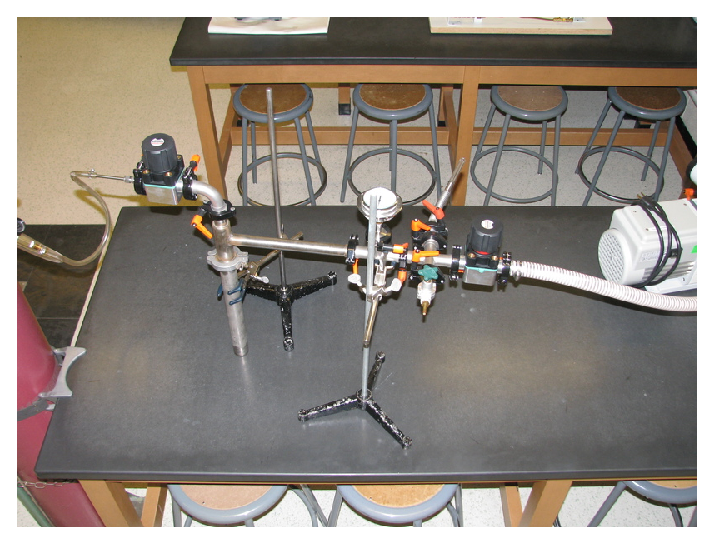
\includegraphics{Leaks-and-Leak-Testing-Table9.eps}
\caption{Leaks and Leak Testing Setup}
\label{fig:VACsetup3}
\end{marginfigure}

\section{Introduction}

One of the major challenges of working with high vacuum systems is assembling a leak free system. In order to reach very low pressure, you must remove or minimize all sources of gas entering the system. Practically speaking there are two types of gas sources. The first is the out-gassing that all physical objects do when pumped down to vacuum pressures. Any object will tend to adsorb gas from its surrounding to a great or lesser extent, and when the gas surrounding the object is removed, the object will gradually give off the gas that it has adsorbed. How much gas is given off, and how long it takes to be given off is very much a function of the object being pumped out. Eventually, surfaces have given off their adsorbed gas and the out-gassing stops or at least is reduced to undetectable amounts.

The other source of gas is actual leaks in the vacuum system. As a vacuum chamber is reduced to lower and lower pressures, the pressure gradient between the inside and the outside of the chamber gets larger and larger. The rate at which gas can leak through a small hole in a chamber wall is dependent both on the size of the hole and on the pressure gradient across the hole. Thus, as the pressure drops, small leaks become more and more important, preventing the system from reaching its lowest possible pressure.

There are a variety of techniques used to look for leaks in a vacuum system. This project will introduce you to some of these methods, including techniques for determining whether or not a leak exists and then trying to find the location of the leak. This exercise provides you with a "leaky" vacuum chamber. The chamber has one or more small leaks, which you can find.

\section{Experimental Procedure}

\begin{figure}
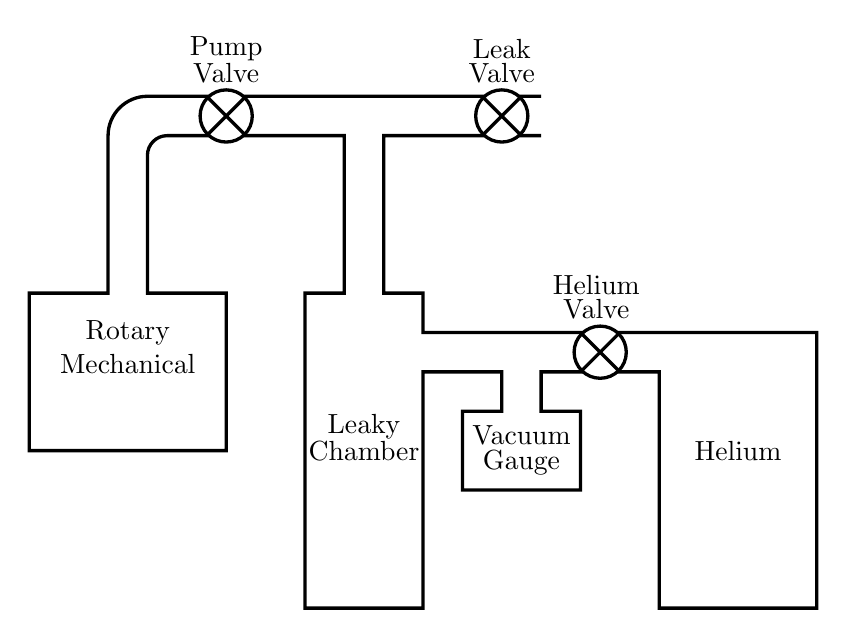
\begin{tikzpicture}
%main body
\draw[very thick](7,7.5)--(2,7.5)arc(90:180:.5)--(1.5,5)--(.5,5)--(.5,3)--(3,3)--(3,5)--
(2,5)--(2,6.75)arc(180:90:.25)--(4.5,7)--(4.5,5)--(4,5)--(4,1)--(5.5,1)--(5.5,4)--(6.5,4)--
(6.5,3.5)--(6,3.5)--(6,2.5)--(7.5,2.5)--(7.5,3.5)--(7,3.5)--(7,4)--(8.5,4)--(8.5,1)--
(10.5,1)--(10.5,4.5)--(5.5,4.5)--(5.5,5)--(5,5)--(5,7)--(7,7);
%valves
\foreach \x/\y in {3/7.25,6.5/7.25,7.75/4.25}{
\begin{scope}
\node[circle,scale=2,draw,fill=white,very thick]at(0+\x,0+\y){};
\draw[very thick](-.25+\x,-.25+\y)--(.25+\x,.25+\y);
\draw[very thick](-.25+\x,.25+\y)--(.25+\x,-.25+\y);
\end{scope}
}
%labels
\node[]at(3,8.1){Pump};
\node[]at(3,7.8){Valve};
\node[]at(6.5,8.1){Leak};
\node[]at(6.5,7.8){Valve};
\node[]at(7.7,5.1){Helium};
\node[]at(7.7,4.8){Valve};
\node[]at(9.5,3){Helium};
\node[]at(6.75,3.2){Vacuum};
\node[]at(6.75,2.85){Gauge};
\node[]at(4.75,3.3){Leaky};
\node[]at(4.75,3){Chamber};
\node[]at(1.75,4.5){Rotary};
\node[]at(1.75,4.1){Mechanical};
\end{tikzpicture}
\caption{Vacuum apparatus.}
\label{fig:vac3}
\end{figure}

\begin{enumerate}
\item Turn on the rotary pump and open the pump valve to evacuate the system.

\item Monitor the pressure with the vacuum gauge. {\bf In your lab notebook, record how long it takes for the system to reach a steady pressure and how low that pressure is.}

\item Close the pump valve and see whether the pressure remains constant or how quickly it changes. Then reopen the pump valve and re-evacuate the chamber.

\item You will now need to work with a high-pressure helium gas line. {\bf \textit{Find a staff member or TA to assist you before proceeding.}} You first want to remove the air from the helium gas line. Make sure the valve on the tank is closed and then open the "helium valve" to evacuate the gas line. Once the pressure has dropped, close the "helium valve" and open the valves on the helium tank itself. Do not change the valve in front of the gauges on the tank, this valve controls the total pressure, and it should already be correctly set.

\item {\bf \textit{Close the pump valve}} and open the helium valve. This will fill your system with slightly over 1 atmosphere of helium. At this point, any leaks will have helium flowing out of them, instead of air into them.

\item Take the "Leak Detective" helium sniffer unit and turn it on. Use the knob on the front to zero the detector so that only a single green light is lit when its detector is well away from any leaks. Take the hand-held nozzle and hold it beside the apparatus, the lights will probably not change. If you move the nozzle near leaking He, then you should see the red LEDs light up indicating that the sniffer has detected excess helium in the air, which is a leak. When you move the nozzle away from the leak and wait for a few seconds the red lights should go out. 

\item There are at least two leaks in the system. Can you find them? Remember, the leaks are quite small, and you need to move the detector nozzle slowly as the system does have a response time. {\bf In your lab notebook, record the location of the leaks.}

\item Once you have found the leaks, be sure to close the helium valve and the two valves on the helium tank (but not the handle that sets the pressure). You can now turn off the pump and immediately fill the chamber and pump with air. If you fail to vent the system, the residual vacuum will actually suck the oil out of the pump and into the pump lines and chamber, making a horrible mess.

\end{enumerate}

\section{IV - Vacuum Manifold and the Pressure Dependence of Altimeters}

\section{Equipment}

% first column
\begin{minipage}[t]{0.5\textwidth}
\begin{itemize}[noitemsep]
\item Vacuum manifold cart
\item Edwards RV3 pump
\end{itemize}
\end{minipage}
%second column
\begin{minipage}[t]{0.5\textwidth}
\begin{itemize}[noitemsep]
\item DC power supply (2)
\item connecting leads
\end{itemize}
\end{minipage}

\begin{marginfigure}
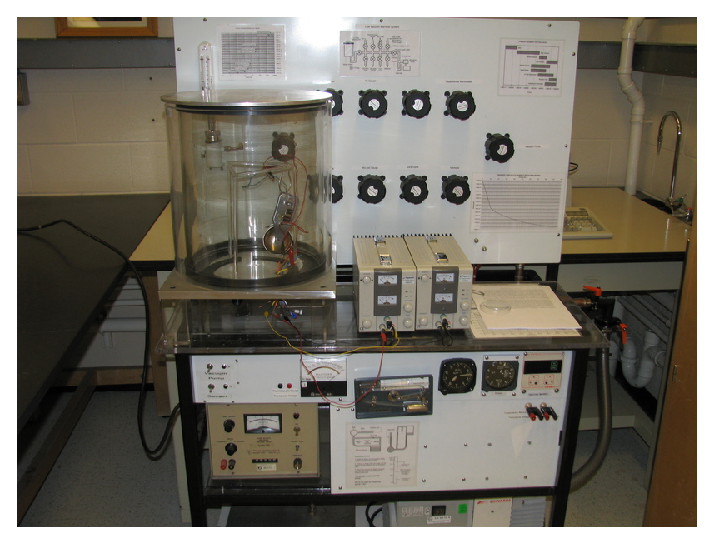
\includegraphics{Manifold-System.eps}
\caption{Manifold Vacuum Setup.}
\label{fig:VACsetup4}
\end{marginfigure}

\section{Introduction}

Air pressure decreases as the altitude increases. This fact forms the basis for the operating principles of conventional altimeters found in airplanes. These mechanical devices measure the atmospheric pressure and then mechanically convert this measurement into an altitude. Altimeters measure the height above sea level, not the height above the ground, so even if you have an altimeter, it is necessary to have some knowledge of the geography over which you are flying or skydiving, to avoid unpleasant ground intercept trajectories.

This experimental project is designed to allow you to determine the dependence between an altimeter reading and actual pressure. Using a vacuum pump, you will lower the pressure of a metal manifold, which has assorted vacuum gauges and an altimeter connected to it. At various times you will stop pumping on the manifold and measure the pressure and altimeter reading, gradually building up a plot that will demonstrate the relationship between these two quantities. 

\section{Experimental Procedure}
\begin{enumerate}
\item Examine the vacuum manifold system in front of you and compare it to the schematic shown in Figure \ref{fig:vac4}. Please ensure that you understand the connections and how to pump out the manifold and control which gauges are connected to it. If you are at all unsure, please go over the system with one of the laboratory staff.


\begin{figure}
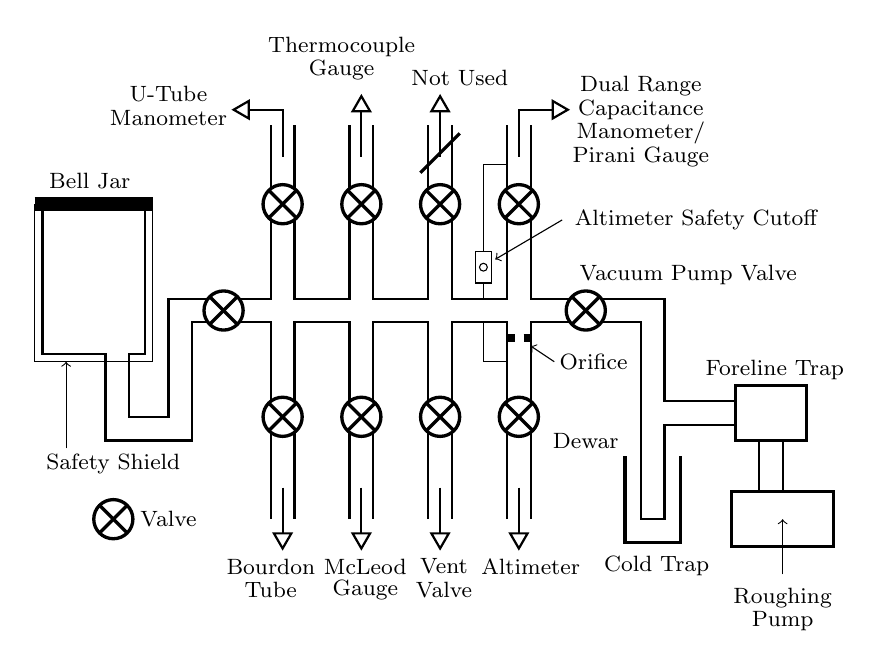
\begin{tikzpicture}
%bell jar
\draw(0,4)rectangle(1.5,6);
\draw[line width=5pt](0,6)--(1.5,6);
\draw[thick](.1,6)--(.1,4.1)--(.9,4.1)--(.9,3)--(2,3)--(2,4.5)--(3,4.5)--(3,2);
\draw[thick](1.4,6)--(1.4,4.1)--(1.2,4.1)--(1.2,3.3)--(1.7,3.3)--(1.7,4.8)--(3,4.8)--(3,7);
\draw[thick](3.3,7)--(3.3,4.8)--(4,4.8)--(4,7);
\draw[thick](4.3,7)--(4.3,4.8)--(5,4.8)--(5,7);
\draw[thick](5.3,7)--(5.3,4.8)--(6,4.8)--(6,7);
\draw[thick](6.3,7)--(6.3,4.8)--(8,4.8)--(8,3.5)--(9.5,3.5)--(9.5,2);
\draw[thick](9.2,2)--(9.2,3.2)--(8,3.2)--(8,2)--(7.7,2)--(7.7,4.5)--(6.3,4.5)--(6.3,2);
\draw[thick](6,2)--(6,4.5)--(5.3,4.5)--(5.3,2);
\draw[thick](5,2)--(5,4.5)--(4.3,4.5)--(4.3,2);
\draw[thick](4,2)--(4,4.5)--(3.3,4.5)--(3.3,2);
\draw[very thick](7.5,2.8)--(7.5,1.7)--(8.2,1.7)--(8.2,2.8);
\node[rectangle,minimum width=1.3cm,minimum height=.7cm,draw,very thick,fill=white]at(9.5,2){};
\node[rectangle,minimum width=.9cm,minimum height=.7cm,draw,very thick,fill=white]at(9.35,3.35){};

%valves
\foreach \x/\y in {2.4/4.65,3.15/6,4.15/6,5.15/6,6.15/6,3.15/3.3,4.15/3.3,5.15/3.3,
6.15/3.3,7/4.65,1/2}{
\begin{scope}
\node[circle,scale=1.5,draw,fill=white,very thick]at(0+\x,0+\y){};
\draw[very thick](-.17+\x,-.17+\y)--(.17+\x,.17+\y);
\draw[very thick](-.17+\x,.17+\y)--(.17+\x,-.17+\y);
\end{scope}
}
%flow arrows
\draw[-open triangle 60,thick](3.15,2.4)--(3.15,1.6);
\draw[-open triangle 60,thick](4.15,2.4)--(4.15,1.6);
\draw[-open triangle 60,thick](5.15,2.4)--(5.15,1.6);
\draw[-open triangle 60,thick](6.15,2.4)--(6.15,1.6);
\draw[-open triangle 60,thick](3.15,6.6)--(3.15,7.2)--(2.5,7.2);
\draw[-open triangle 60,thick](4.15,6.6)--(4.15,7.4);
\draw[-open triangle 60,thick](5.15,6.6)--(5.15,7.4);
\draw[-open triangle 60,thick](6.15,6.6)--(6.15,7.2)--(6.8,7.2);
%altimeter safety cutoff
\draw[thin](6,6.5)--(5.7,6.5)--(5.7,4.8);
\draw[thin](5.7,4.5)--(5.7,4)--(6,4);
\draw[fill=white](5.6,5)rectangle(5.8,5.4);
\node[circle,scale=.3,draw]at(5.7,5.2){};
\draw[dashed,line width=3pt](6,4.3)--(6.3,4.3);
%labels
\draw[very thick](4.9,6.4)--(5.4,6.9);
\node[font=\footnotesize]at(1.7,2){Valve};
\node[font=\footnotesize]at(.7,6.3){Bell Jar};
\node[font=\footnotesize]at(1,2.7){Safety Shield};
\draw[thin,->](.4,2.9)--(.4,4);
\node[font=\footnotesize]at(6.3,1.4){Altimeter};
\node[font=\footnotesize]at(7.9,1.4){Cold Trap};
\node[font=\footnotesize]at(9.4,3.9){Foreline Trap};
\node[font=\footnotesize]at(5.4,7.6){Not Used};
\node[font=\footnotesize]at(7.1,4){Orifice};
\draw[thin,->](6.6,4)--(6.3,4.2);
\node[font=\footnotesize]at(7,3){Dewar};
\node[font=\footnotesize]at(9.5,1){Roughing};
\node[font=\footnotesize]at(9.5,.7){Pump};
\draw[thin,->](9.5,1.3)--(9.5,2);
\node[font=\footnotesize]at(8.3,5.1){Vacuum Pump Valve};
\node[font=\footnotesize]at(5.2,1.4){Vent};
\node[font=\footnotesize]at(5.2,1.1){Valve};
\node[font=\footnotesize]at(4.2,1.4){McLeod};
\node[font=\footnotesize]at(4.2,1.1){Gauge};
\node[font=\footnotesize]at(3,1.4){Bourdon};
\node[font=\footnotesize]at(3,1.1){Tube};
\node[font=\footnotesize]at(1.7,7.4){U-Tube};
\node[font=\footnotesize]at(1.7,7.1){Manometer};
\node[font=\footnotesize]at(3.9,8){Thermocouple};
\node[font=\footnotesize]at(3.9,7.7){Gauge};
\node[font=\footnotesize]at(7.7,7.5){Dual Range};
\node[font=\footnotesize]at(7.7,7.2){Capacitance};
\node[font=\footnotesize]at(7.7,6.9){Manometer/};
\node[font=\footnotesize]at(7.7,6.6){Pirani Gauge};
\node[font=\footnotesize]at(8.4,5.8){Altimeter Safety Cutoff};
\draw[thin,->](6.7,5.8)--(5.85,5.3);
\end{tikzpicture}
\caption{Schematic of vacuum manifold system.}
\label{fig:vac4}
\end{figure}


\item Open the valve that connects the altimeter and capacitance manometer to the vacuum manifold. Ensure that the manifold is at atmospheric pressure and record the pressure and altitude readings.   

\item Ensure that the vent valve for the mechanical pump is closed and then turn on this rotary vane mechanical pump, which you will be using to evacuate the manifold.  

\item Slowly open the main pumping valve to evacuate some air from the manifold. Close the valve as soon as the pressure has changed significantly. {\bf In your lab notebook, record the pressure and altimeter reading and then repeat the process to further lower the pressure.}  Continue until the pressure and or altimeter reading is no longer changing. (Note: the maximum altitude that you will achieve is in the neighbourhood of 45000 feet due to a protection relay device inside the altimeter.)

\item {\bf Generate a plot of pressure versus altitude reading using your data and include it in your lab notebook.} If you feel that your data is insufficient you can bring the manifold up to atmospheric pressure again (consult the staff about this if you are at all unsure) and then collect more pressure-altitude data as described in Step 4.

\item Take a moment to look at your data and consider what sort of functional dependence the pressure has on the altitude. Does this dependence make sense? If you are twice as high is the pressure half as much? more? less?
\end{enumerate}

\section{V - Assembly of a Low Vacuum System}

\section{Equipment}

% first column
\begin{minipage}[t]{0.5\textwidth}
\begin{itemize}[noitemsep]
\item Edwards RV3 pump
\item Isolation valve (2)
\item Vacuum hose
\item 25 cm tube with NW25 terminations
\item Four-way cross with NW25 flanges
\end{itemize}
\end{minipage}
%second column
\begin{minipage}[t]{0.5\textwidth}
\begin{itemize}[noitemsep]
\item Varian vacuum gauge and gauge head
\item assortment of NW25 rubber O-rings and metal centering rings
\item foreline trap
\item Assortment of NW25 clamps
\item Rubber gloves
\end{itemize}
\end{minipage}

\begin{marginfigure}
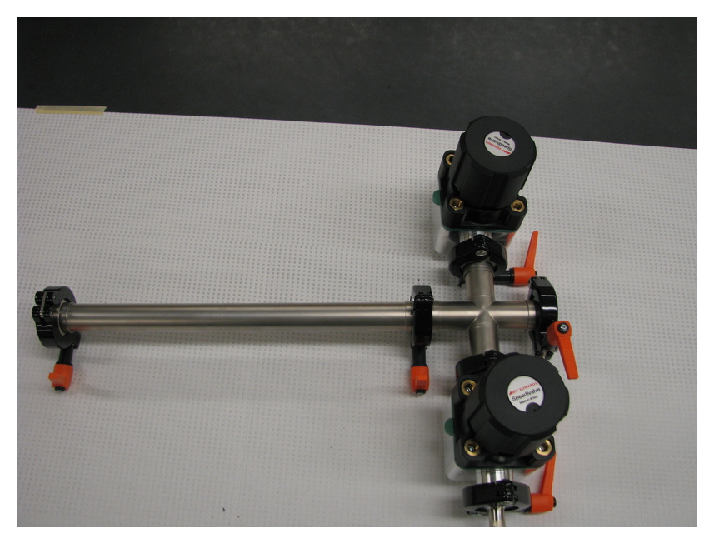
\includegraphics{Low-Vacuum-System-Assembled-Table1-2.eps}
\caption{Assembly of Low Vacuum Setup}
\label{fig:VACsetup5}
\end{marginfigure}

\section{Introduction}

A basic vacuum system consists of a pump to generate the vacuum, a hose to connect the vacuum pump to the process chamber, and gaskets to seal the connections. Additionally, one would probably add a vacuum gauge to measure the pressure in the system and a foreline trap to prevent oil vapour produced by the oil-sealed rotary pump from migrating into the vacuum chamber. Vacuum valves may be inserted in the vacuum system to isolate the process chamber from the vacuum pump as well as enabling the system to be brought back up to atmospheric pressure.  

Your goal in this exercise is to assemble a vacuum system, generate a vacuum in the chamber, measure the ultimate pressure, and then bring the system back to atmospheric pressure. Your system should feature:
\begin{enumerate}[label={(\arabic*)}]
\item a foreline trap,
\item an isolation valve between the vacuum pump and the process chamber,
\item an isolation valve to bring the system back to atmospheric pressure, and
\item a thermocouple gauge to measure the pressure in the system. 
\end{enumerate}
Keep in mind that the presence of water vapour and oils from your fingers will outgas in the vacuum and limit the lowest pressure your system will achieve. Therefore, always handle vacuum components with gloves.

In your design of the vacuum system, keep in mind that corners and narrow diameter vacuum lines will degrade the pumping speed. Keep the number of connections to a minimum as every connector is a potential source of an air leak. The foreline trap should be located as close to the oil-sealed rotary pump as possible.

\section{Experimental Procedure}
\begin{enumerate}
\item {\bf Draw a schematic diagram of your proposed vacuum system.}  Make sure to label each component.

\item {\bf In point form, describe how you will operate your vacuum system, including the initial start-up, operation, and venting.}  It is important that you consider the order that the isolation valves are open or closed when starting and venting the system.  Remember that vacuum pumps should never be left pumping on air at atmospheric pressure for long periods of time.  This will eventually break down the oil and damage the pump.

\item Assemble the system that you have designed.

\item Following your instructions, start the vacuum pump. {\bf Record the lowest pressure that you are able to generate in the vacuum system.}

\item After a couple of minutes at a stable pressure, bring the system back up the atmospheric pressure.

\item Disassemble the vacuum system, ready for the next group to work with.
\end{enumerate}

\section{VI - Pump Down Curves}

\section{Equipment}

% first column
\begin{minipage}[t]{0.5\textwidth}
\begin{itemize}[noitemsep]
\item Vernier data acquisition system with printer support
\item Vernier instrumentation amplifier
\item pumpdown\_template.cmbl Loggerpro file
\end{itemize}
\end{minipage}
%second column
\begin{minipage}[t]{0.5\textwidth}
\begin{itemize}[noitemsep]
\item Pumpdown and leakout curve apparatus
\item Stopwatch
\end{itemize}
\end{minipage}

\begin{marginfigure}
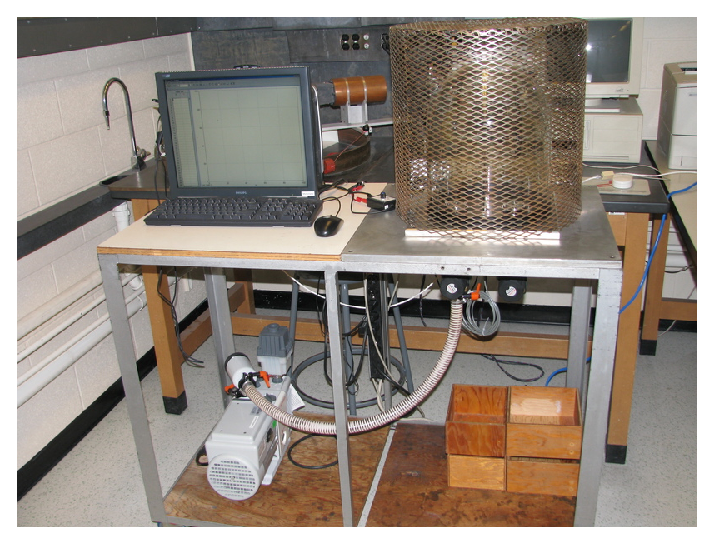
\includegraphics{Pump-Down-Curves.eps}
\caption{Pump Down Curve Setup}
\label{fig:VACsetup6}
\end{marginfigure}

\section{Introduction}

The amount of flow in a vacuum can be described by two quantities commonly used in fluid mechanics, {\bf volumetric flow}, and the {\bf throughput}. Volumetric flow, S, is the net volume of gas that passes through a given area in a unit time and is expressed in units of m$^3\times$s$^{-1}$. The throughput, Q, is the number of molecules that pass through a channel in a unit time and is expressed in units of Pa$\times$m$^3\times$s$^{-1}$. Since the number of molecules in a unit volume of gas is directly proportional to the pressure, the throughput can be represented mathematically as

\begin{equation}
Q=PS
\label{equ:vac1}
\end{equation}

\begin{marginfigure}
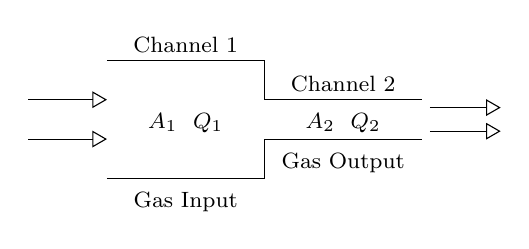
\begin{tikzpicture}
\draw[](1,3)--(3,3)--(3,2.5)--(5,2.5); %channels
\draw[](1,1.5)--(3,1.5)--(3,2)--(5,2); %gas input/output
%arrows
\draw[-open triangle 60](0,2)--(1,2);
\draw[-open triangle 60](0,2.5)--(1,2.5);
\draw[-open triangle 60](5.1,2.1)--(6,2.1);
\draw[-open triangle 60](5.1,2.4)--(6,2.4);
%labels
\node[font=\footnotesize]at(2,3.2){Channel 1};
\node[font=\footnotesize]at(4,2.7){Channel 2};
\node[font=\footnotesize]at(2,1.2){Gas Input};
\node[font=\footnotesize]at(4,1.7){Gas Output};
\node[font=\footnotesize]at(2,2.2){$A_1$\hspace{2mm}$Q_1$};
\node[font=\footnotesize]at(4,2.2){$A_2$\hspace{2mm}$Q_2$};
\end{tikzpicture}
\caption{}
\label{fig:vac5}
\end{marginfigure}

Due to the {\bf conservation of mass}, throughput is always {\bf conserved} when dealing with flow through geometries of different sizes. Figure \ref{fig:vac5} shows a channel whose geometry varies in size at some point where A1 is the area of the larger portion of the channel and A2 is the area of the smaller portion. Providing that the temperature of the gas remains unchanged the number of molecules that pass into the smaller chamber remains constant, conserving the throughput even though the volume of the channel changes with length. Therefore, the gas output is equal to the gas input in this portion of the channel and hence

\begin{equation}
Q_1=Q_2=Q
\label{equ:vac2}
\end{equation}

\noindent for the entire length of the channel.

\begin{marginfigure}
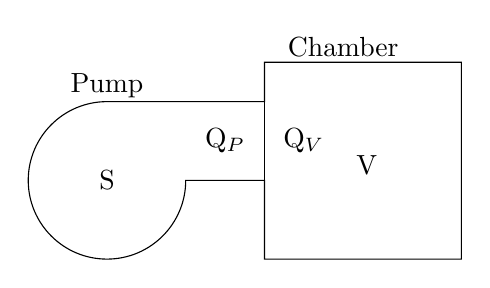
\begin{tikzpicture}
\draw[](1,3)arc(90:360:1)--(3,2)--(3,1)--(5.5,1)--(5.5,3.5)--(3,3.5)--(3,3)--(1,3);
\draw[](3,3)--(3,2);
%labels
\node[]at(1,3.2){Pump};
\node[]at(4,3.7){Chamber};
\node[]at(1,2){S};
\node[]at(2.5,2.5){Q$_P$};
\node[]at(3.5,2.5){Q$_V$};
\node[]at(4.3,2.2){V};
\end{tikzpicture}
\caption{}
\label{fig:vac6}
\end{marginfigure}

Pumps are designed to remove gas from the system at a constant volumetric flow rate or an {\bf effective pumping speed} of the system. For a given throughput and lowest system pressure required, it is possible to use Equation \ref{equ:vac1} to estimate the pumping speed needed to achieve that pressure.

The throughput of a vacuum system allows for the derivation of the rate in which the pressure will decrease when it is being pumped on. This {\bf pumpdown rate} can be derived by considering the throughput of gas from a chamber into a pump. Figure \ref{fig:vac6} shows a pump that is attached to an enclosed chamber of volume V. Assume that there is a perfect seal between the pump and the chamber so that all of the gas leaving the chamber goes directly into the pump. Since the volume of the chamber remains constant, the throughput of the gas leaving the volume, Q$_V$, changes only due to the varying pressure of the system such that 

\begin{equation}
Q_V=-V\dfrac{dP}{dt}
\label{equ:vac3}
\end{equation}

\noindent The negative sign arises since the pressure in the chamber is decreasing with time.

The throughput on the pump side, Q$_P$, is the amount of gas that is entering the pump and is given by Equation \ref{equ:vac4}. Note that in this case S represents the speed of the pump. Combining Equations \ref{equ:vac1}, \ref{equ:vac2}, and \ref{equ:vac3} results in

\begin{equation}
\dfrac{dP}{dt}+\dfrac{S}{V}P=0
\label{equ:vac4}
\end{equation}

\noindent This is a first order linear differential equation with the exponential solution

\begin{equation}
P(t)=P_0e^{-\frac{S}{V}t}
\label{equ:vac5}
\end{equation}

\noindent where t is the time to pump down to the pressure P, and P$_0$ is the initial pressure of the chamber. From this equation, it can be seen that the pressure of a vacuum system decreases exponentially with time as it is pumped down. Due to the fact that this is an exponential decrease, a plot of pressure versus time for a system pumpdown is often referred to as the {\bf pumpdown curve}. Note that for most vacuum systems S is assumed to remain constant with time. Therefore, since the volume of the chamber does not change, the S/V term in the exponential is a constant that is characteristic of the particular vacuum system, including both the pump and the enclosed volume.

The apparatus used in this experiment can be seen in Figure \ref{fig:vac7}. It consists of a {\bf Bell Jar}, which acts as the process chamber for this vacuum system. The chamber is connected to a pump by means of a long tube. A foreline trap is placed between the pump and the connecting tube.

The base of this system is constructed from a stainless steel plate. The bottom of the bell jar is lined with rubber which creates a seal between the jar and the base. The tube connecting the pump to the chamber is fed through the bottom of the base plate and into the Bell jar. Whenever a piece of glass is placed under vacuum there is a chance that the glass could implode due to the pressure. As a safety precaution, whenever the bell jar is being pumped down below atmospheric pressure always ensure that it is covered with the protective steel shielding.

\begin{figure}
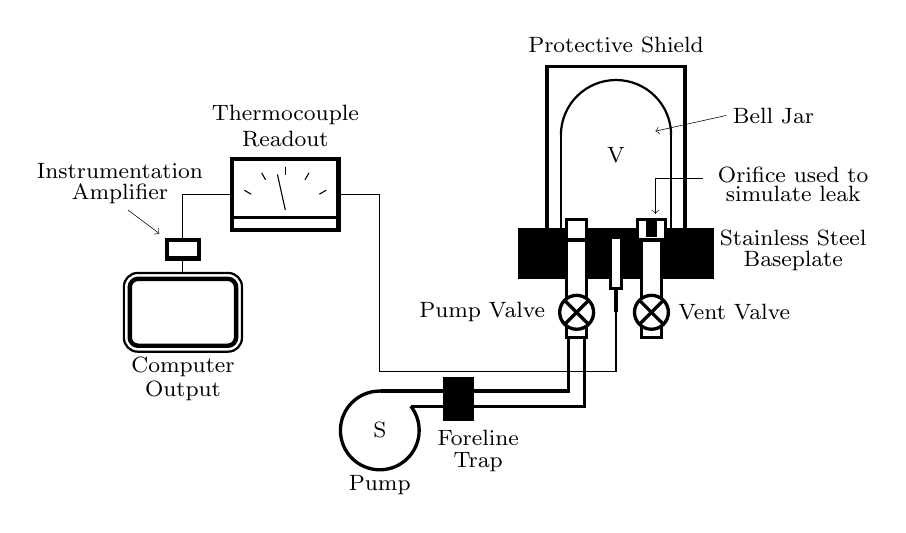
\begin{tikzpicture}
\draw[](2,4)--(2,5.5)--(4.5,5.5)--(4.5,3.25)--(7.5,3.25)--(7.5,4.5);%circuit
%computer output
\node[rectangle,fill=white,draw,rounded corners=5pt,minimum width=1.5cm,minimum height=1cm,thick]at(2,4){};
\node[rectangle,fill=white,draw,rounded corners=3pt,minimum width=1.35cm,minimum height=.85cm,ultra thick]at(2,4){};
%thermocouple readout
\node[rectangle,fill=white,draw,minimum width=1.35cm,minimum height=.9cm,line width=1.5pt]at(3.3,5.5){};
\draw[very thick](2.6,5.2)--(4,5.2);
\draw(3.3,5.3)--(3.2,5.75); %pointer
\begin{scope}[shift={(3.3,5.25)}]
\foreach \r in {-60,-30,0,30,60}{
\draw[thin,rotate=\r](0,.5)--(0,.6);}
\end{scope}
%jar assembly
\node[rectangle,minimum width=1.75cm,minimum height=2.25cm,fill=white,very thick,draw]at(7.5,6){};
\node[rectangle,minimum width=2.5cm,minimum height=.65cm,fill]at(7.5,4.75){};
\draw[thick](6.8,5)--(6.8,6.25);
\draw[thick](8.2,5)--(8.2,6.25);
\draw[thick](6.8,6.25) arc(180:0:.7);
\draw[fill=white,draw,very thick](7.43,4.3)rectangle(7.57,4.95);
\draw[ultra thick](7.5,4)--(7.5,4.3);
%pump conduit
\node[rectangle,minimum width=.25cm,minimum height=.25cm,fill=white,very thick,draw]at(7,5.05){};
\node[rectangle,minimum width=.25cm,minimum height=1.24cm,fill=white,very thick,draw]at(7,4.3){};
\node[circle,fill=white,very thick,scale=1.3,draw]at(7,4){}; %pump valve
\draw[very thick](6.85,3.85)--(7.15,4.15); %pump valve
\draw[very thick](6.85,4.15)--(7.15,3.85); %pump valve
\draw[very thick](4.5,3)--(6.9,3)--(6.9,3.68)--(7.1,3.68)--(7.1,2.8)--(4.9,2.8);
\draw[very thick](4.5,3) arc(-270:38:.5);
\node[rectangle,minimum width=.4cm,minimum height=.55cm,fill]at(5.5,2.9){}; %foreline trap
%vent assembly
\node[rectangle,minimum width=.35cm,minimum height=.25cm,fill=white,very thick,draw]at(7.95,5.05){};
\node[rectangle,minimum width=.25cm,minimum height=1.24cm,fill=white,very thick,draw]at(7.95,4.3){};
\draw[line width=4pt](7.95,5.2)--(7.95,4.95);
\node[circle,fill=white,very thick,scale=1.3,draw]at(7.95,4){}; %vent valve
\draw[very thick](7.8,3.85)--(8.1,4.15); %vent valve
\draw[very thick](7.8,4.15)--(8.1,3.85); %vent valve
%amplifier
\node[rectangle,fill=white,draw,minimum width=4mm,minimum height=2mm,line width=1.5pt]at(2,4.8){};
%labels
\node[font=\footnotesize]at(1.2,5.8){Instrumentation};
\node[font=\footnotesize]at(1.2,5.5){Amplifier};
\draw[very thin,->](1.3,5.3)--(1.7,5);
\node[font=\footnotesize]at(2,3.3){Computer};
\node[font=\footnotesize]at(2,3){Output};
\node[font=\footnotesize]at(3.3,6.5){Thermocouple};
\node[font=\footnotesize]at(3.3,6.2){Readout};
\node[font=\footnotesize]at(7.5,7.4){Protective Shield};
\node[font=\footnotesize]at(5.8,4){Pump Valve};
\node[font=\footnotesize]at(9,4){Vent Valve};
\node[font=\footnotesize]at(4.5,2.5){S};
\node[font=\footnotesize]at(4.5,1.8){Pump};
\node[font=\footnotesize]at(5.75,2.4){Foreline};
\node[font=\footnotesize]at(5.75,2.1){Trap};
\node[font=\footnotesize]at(7.5,6){V};
\node[font=\footnotesize]at(9.5,6.5){Bell Jar};
\draw[very thin,->](8.9,6.5)--(8,6.3);
\node[font=\footnotesize]at(9.75,5.75){Orifice used to};
\node[font=\footnotesize]at(9.75,5.5){simulate leak};
\draw[very thin,->](8.6,5.7)--(8,5.7)--(8,5.25);
\node[font=\footnotesize]at(9.75,4.95){Stainless Steel};
\node[font=\footnotesize]at(9.75,4.65){Baseplate};
\end{tikzpicture}
\caption{A schematic of the set up for a bell jar vacuum system with pump and instrumentation.}
\label{fig:vac7}
\end{figure}

A {\bf thermocouple gauge} attached to the base of the Bell Jar measures the pressure of the system. A computer equipped with an analog-to-digital converter, instrumentation amplifier, and LoggerPro software records the voltage output of the thermocouple gauge.

\section{Experimental Procedure}
\begin{enumerate}
\item Before beginning, ensure that the protective steel caging is placed over the Bell jar. This is absolutely necessary since any piece of glass placed under vacuum has a risk of imploding. If the protective steel caging is not on the Bell jar, consult the TA before continuing.

\item Start the vacuum pump.

\item Start the Loggerpro software on the computer and load the pumpdown\_template.cmbl file located on the desktop. After the file has been loaded a window will appear prompting you to connect the instrumentation amplifier to that computer. Set the instrumentation amplifier to 0-20 mV. Click on the "connect" button located in the lower right corner of the screen, then click ok.

\item Vent the Bell jar by first closing the pump valve and then opening up the vent valve. Leave the vent valve open with the pump valve closed for about 2 minutes to allow the Bell jar time to return to atmospheric pressure.

\item Close the vent valve and then start the data collection in Loggerpro. Once the computer has started collecting data open up the pump valve to allow the system to pump down.

\item Allow the system to pump down for roughly 15 minutes, at which point the system should approximately be at a pressure of 100 millitorr. {\bf At this point measure the pressure of the system using the output on the Loggerpro software and record this as the ultimate pressure of the system.} At any point during the operation of the software the scales on the graphs can be manipulated by moving the mouse cursor over the graph until it turns into a cross and double clicking. Under the Axes Options tab the scales can either be entered manually or set to autoscale. Note that the autoscaling feature will only work while data is being collected. After the data acquisition has ceased the scales will have to be set manually.

\item Stop the data collection in LoggerPro and set the maximum and minimum for pressure on the pumpdown curve to be 2000 millitorr and 0 millitorr respectively. Once this has been done, {\bf fit an exponential to the graph.} To fit an exponential to the pumpdown curve, the appropriate region of the graph should be highlighted with a grey box using the mouse. Note that there are two shades of grey that are used to select the graph. The lighter shade of grey confines only the horizontal region while the darker grey box includes both the horizontal and vertical regions of the selected portion of the graph. After the region has been selected, click the "Curve Fit" button at the top of the screen. Under the list of predefined functions select the combo box with the equation A*exp(-Ct)+B.

\item {\bf Print a copy of the pumpdown curve you determined for the vacuum system.} To print the graph, select the box containing the graph by clicking on the white space outside of the axes to highlight it. After the graph has been selected, go to the File menu and select the "Print Graph" option located near the bottom of the menu.

\item Switch off the vacuum pump and vent the Bell jar.
\end{enumerate}

The Physics Junior Laboratory operates two systems that demonstrate how a high vacuum system may be generated by an oil diffusion pump and a turbo molecular pump. These systems are available for you to explore. Please contact a TA if you would like to have a closer look. High vacuum systems are more complex than the systems you have encountered to this point and can be easily damaged if you are not experienced with their operation.

\section{VII - Diffstak System and Leak Rates}

\section{Equipment}

% first column
\begin{minipage}[t]{0.5\textwidth}
\begin{itemize}[noitemsep]
\item Diffstak equipment cart
\item RG-83 ionization gauge controller
\end{itemize}
\end{minipage}
%second column
\begin{minipage}[t]{0.5\textwidth}
\begin{itemize}[noitemsep]
\item Edwards RV5 vacuum pump
\end{itemize}
\end{minipage}

\begin{marginfigure}
\includegraphics{diffstak.jpg}
\caption{A photograph of the experimental setup.}
\label{fig:VACsetup7}
\end{marginfigure}

\section{Introduction}

Diffstak diffusion pumps are among the most common designs for commercial oil diffusion pumps. It is a multistage pump, with the stages stacked one on to of the other in a stack, called a Diffstak. This arrangement is available for you to look at.

Oil diffusion pumps are commonly used to reach medium to high vacuum levels with  $10^{-6}$ to $10^{-7}$ Torr easily achievable, and even lower pressures possible with specially designed systems. Diffusion pumps are probably the most efficient pumping system for removing light atoms such as hydrogen, but it has the disadvantage of generating a "dirtier" vacuum, due to oil back flow, compared to turbo molecular or ion-getter pumps. This effect can be minimized by the addition of a baffled liquid nitrogen trap, which reduces the pumping speed somewhat, but greatly improves the quality of the vacuum by condensing oil vapour that might flow back from the pump to the chamber.

Diffstak diffusion pumps are classified by their inside diameter, with the smallest pumps being as small as 1" diameter. Large pumps, up to 18" in diameter and larger, are commonly available for use with large vacuum systems.  2", 4", and 6" diffusion pumps can be found in the Physics and Astronomy Department. The unit you will be using is a 3" pump.

The purpose of this laboratory is to introduce you to the Diffstak pumps and two types of vacuum gauges (thermocouple and ionization). Thermocouple gauges are useful for measure low quality vacuums. They, like the related Pirani Gauges, work by measuring the change in thermal conductivity in a gas as the pressure changes. With a thermocouple gauge, a current is run through a thermocouple junction positioned inside the vacuum. This heats up the wire, generating a DC potential in the thermocouple. When the pressure falls, less heat is dissipated from the wire, resulting in a higher temperature in the thermocouple, and thus a larger DC potential. The control unit measures the DC potential and converts it into an absolute pressure reading. Thermocouple gauges are accurate from nearly an atmosphere down to roughly 1 mTorr. At lower pressures, an ionization gauge is commonly used to measure pressures.

The ionization gauge operates by generating free electrons from an electrically-heated filament. These electrons collide with atoms in the low-pressure gas, generating ions. A negatively biased collection electrode attracts the positively charge ions but repels the electrons.  The control unit simply counts the number of ions, actually the number of charges, hitting the collection electrode. At low enough pressures the dependence of the electrode current is relatively simple: higher pressure means more atoms and molecules to ionize which yields a larger current. These gauges work from roughly $10^{-3}$ Torr down below $10^{-10}$ Torr. At times contaminants collect in the gauge heads, and at very low pressures these contaminants can lead to erroneously high pressure readings. Therefore, these gauges have a feature known as outgassing, in which a heating filament raises the temperature of the gauge head, in an effort to remove most of the contaminants.

To the frustration of every experimenter, all vacuum systems leak at some rate, however small. In general, the pump overcomes this leak rate. In order to observe a leak rate, one simply isolates the chamber of interest from all vacuum pumps, and observes how rapidly the pressure rises. Alternately, one can then open up the pump valves, and determine how quickly the pressure falls, determining the pumping rate. Figure \ref{fig:vac8} diagrams the experimental apparatus, and labels the valves, defining the terminology used in the following experimental procedure descriptions.

\section{Experimental Procedure}

\begin{figure}
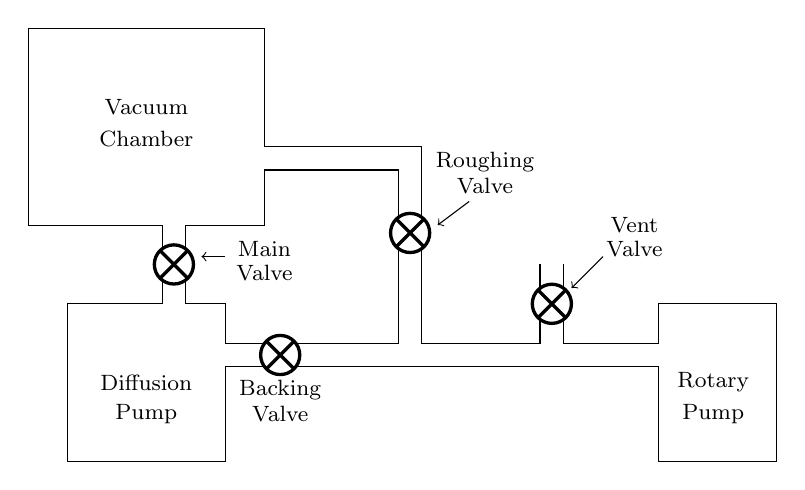
\begin{tikzpicture}
\draw[](0,7)--(3,7)--(3,5.5)--(5,5.5)--(5,3)--(6.5,3)--(6.5,4);
\draw[](6.8,4)--(6.8,3)--(8,3)--(8,3.5)--(9.5,3.5)--(9.5,1.5)--(8,1.5)--
(8,2.7)--(2.5,2.7)--(2.5,1.5)--(.5,1.5)--(.5,3.5)--(1.7,3.5)--(1.7,4.5)--
(0,4.5)--(0,7);
\draw[](3,5.2)--(4.7,5.2)--(4.7,3)--(2.5,3)--(2.5,3.5)--(2,3.5)--(2,4.5)--
(3,4.5)--(3,5.2);
%valves
\foreach \x/\y in {1.85/4,3.2/2.85,4.85/4.4,6.65/3.5}{
\begin{scope}
\node[circle,scale=1.5,draw,fill=white,very thick]at(0+\x,0+\y){};
\draw[very thick](-.17+\x,-.17+\y)--(.17+\x,.17+\y);
\draw[very thick](-.17+\x,.17+\y)--(.17+\x,-.17+\y);
\end{scope}
}
%labels
\node[font=\footnotesize]at(1.5,6){Vacuum};
\node[font=\footnotesize]at(1.5,5.6){Chamber};
\node[font=\footnotesize]at(1.5,2.5){Diffusion};
\node[font=\footnotesize]at(1.5,2.1){Pump};
\node[font=\footnotesize]at(8.7,2.5){Rotary};
\node[font=\footnotesize]at(8.7,2.1){Pump};
\node[font=\footnotesize]at(3,4.2){Main};
\node[font=\footnotesize]at(3,3.9){Valve};
\draw[->](2.5,4.1)--(2.2,4.1);
\node[font=\footnotesize]at(3.2,2.4){Backing};
\node[font=\footnotesize]at(3.2,2.1){Valve};
\node[font=\footnotesize]at(5.8,5.3){Roughing};
\node[font=\footnotesize]at(5.8,5){Valve};
\draw[->](5.6,4.8)--(5.2,4.5);
\node[font=\footnotesize]at(7.7,4.5){Vent};
\node[font=\footnotesize]at(7.7,4.2){Valve};
\draw[->](7.3,4.1)--(6.9,3.7);
\end{tikzpicture}
\caption{Diagram of the vacuum apparatus.}
\label{fig:vac8}
\end{figure}

There are two rules that you must follow while working with this system:

\indent {\bf Rule \#1:} never expose an operating diffusion pump to atmospheric pressure.
\indent {\bf Rule \#2:} never have both the roughing valve and the backing valve, or both the roughing and the main valve open at the same time.

\section{VIII - High Vacuum Turbo Molecular System}

\section{Equipment}

% first column
\begin{minipage}[t]{0.5\textwidth}
\begin{itemize}[noitemsep]
\item Turbo V80 pump cart
\end{itemize}
\end{minipage}
%second column
\begin{minipage}[t]{0.5\textwidth}
\begin{itemize}[noitemsep]
\item Edwards RV5 vacuum pump
\end{itemize}
\end{minipage}

\begin{marginfigure}
\includegraphics{turbo-pump-system.jpg}
\caption{A photograph of the experimental setup.}
\label{fig:VACsetup8}
\end{marginfigure}

\section{Introduction}

Many of us are familiar with thinking about gases as fluids that flow from high-pressure regions to low pressure regions. As one decreases the pressure, gases cease to behave as conventional fluids. At atmospheric pressure (760 Torr), the mean free path of an atom or molecule (average distance it travels between collisions with other atoms or molecules) is only a few tens of microns, and even at 1 Torr the mean free path is only a few mm. However, at $10^{-6}$ Torr, the mean free path has reached 51 m, and the particles travel as projectiles, crossing chambers in straight lines and bouncing off chamber walls rather than other atoms. At these low pressures, the gas no longer flows into regions of lower pressure, so mechanical rotary pumps are ineffective. Instead, one uses a projectile approach to lowering the pressure. For example, if you can hit an atom towards the exhaust of the chamber, one can reduce the atomic density.  This is the basic principle of operation of a turbo molecular pump. It looks very much like a turbojet mounted on the side of your vacuum chambers. It has a series of very fast spinning rotor blades angled so that when they strike atoms they drive them down the turbo-pump, where further blades keep the atoms moving downwards. This device will in fact concentrate the atoms to the point where a conventional rotary pump can removed the compressed gas out of turbo molecular pump. Turbo molecular pumps are always operated in series with rotary pumps.

The demonstration consists of a vacuum chamber, turbo molecular pump, and rotary pump. This system has an ionization gauge to measure the pressure in the vacuum chamber.  Compare the pressure in the chamber pumped by the turbo molecular pump to that measured in the system pumped by the oil diffusion pump. 

Unfortunately, due to the high cost and relatively sensitive nature of these pumps, we cannot let everyone try operating these systems for themselves. In addition, on a high vacuum scale, metal actually looks like a sponge, absorbing and "outgassing" atoms and molecules.  Whenever such a system is exposed to air, the metal surfaces adsorb the atoms and molecules.  It then takes a long time to pump the system to very low pressures since the metal surfaces themselves give off gas for quite a long time period. Therefore, we cannot keep re-opening the vacuum chamber and still achieve very low pressures. 



\AtEndDocument{\clearpage\ifodd\value{page}\else\null\clearpage\fi} % forces even page count, for double siding

%%%end document%%% DO NOT REMOVE THIS LINE

\end{document}
